\documentclass[journal, spanish]{IEEEtran}

% Paquetes necesarios
\usepackage[T1]{fontenc}
\usepackage[utf8]{inputenc}
\usepackage{babel}
\usepackage{graphicx}
\usepackage{float}

% Configuración de las cabeceras
\markboth{Diseño de interfaces}{Base de datos}


% Configuración de las secciones
\title{Analisis bibliográfico}
\author{Alejandra Hernández Bermeo\thanks{} \\
\textit{Fundación universitaria Konrad Lorenz} \\
}
\begin{document}

% Creación del título
\maketitle

% Creación del abstract
\begin{abstract}
En este documento se mostrata el analisis bibliografico que le realiace en la base de datos Scopus sobre API
\end{abstract}

% Introducción
\section{Introducción}
Este artículo muestra un análisis bibliográfico de literatura científica reciente sobre las interfaces de programación de aplicaciones (API). La investigación se enfoca en identificar los principales temas y tendencias de investigación en esta área que plantean las API en el contexto actual de la tecnología. Se revisaron una selección de artículos académicos publicados entre 2011 y 2023 en revistas de ingeniería con la palabra clave exacta "Application Programming Interfaces (API)".

Se encuentra una vista general de las principales áreas de investigación relacionadas con las API, incluyendo su implementación, integración, rendimiento, seguridad y privacidad.

% Resultados
\section{Resultados}
Con el query resultante se logro una búsqueda de artículos académicos publicados en revistas de ingeniería que utilizan sistemas de datos y API (interfaces de programación de aplicaciones), publicados entre 2011 y 2023 en inglés y con la palabra clave exacta "Application Programming Interfaces (API)". Además, se limita la búsqueda a artículos de acceso abierto excluyendo la categoría de física.

Como resultado se obtienen los siguientes tipos de articulos:

1. Artículos que analicen la implementación de API en sistemas de datos específicos, como bases de datos, redes sociales, etc.

2. Investigaciones que evalúen el rendimiento y la eficiencia de las API en diferentes contextos.

3. Estudios que aborden la seguridad y la privacidad en el uso de API en sistemas de datos.

4. Investigaciones que aborden la integración de API en sistemas ya existentes, como aplicaciones móviles, software empresarial, etc.

5. Artículos que aborden el impacto de las API en la innovación y el desarrollo tecnológico.


\subsection{Flujo del Analisis}

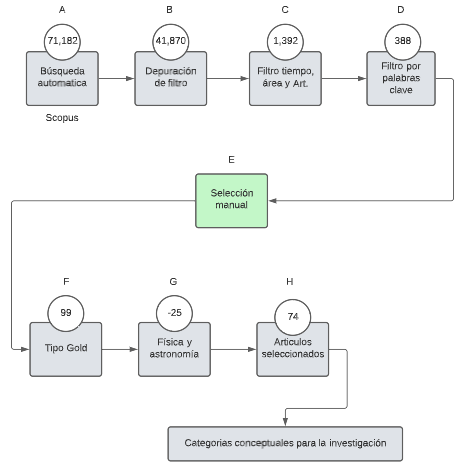
\includegraphics[width=0.4\textwidth]{images/flujo .png}
\subsection{Query Exploratoria}

TITLE-ABS-KEY ( api ) AND PUBYEAR > 2010 AND PUBYEAR < 2024 AND ( LIMIT-TO ( SUBJAREA , "ENGI" ) ) AND ( LIMIT-TO ( DOCTYPE , "ar" ) ) AND ( LIMIT-TO ( EXACTKEYWORD , "Application Programming Interfaces (API)" ) ) AND ( LIMIT-TO ( LANGUAGE , "English" ) )


\subsection{Analisis de Titulo}

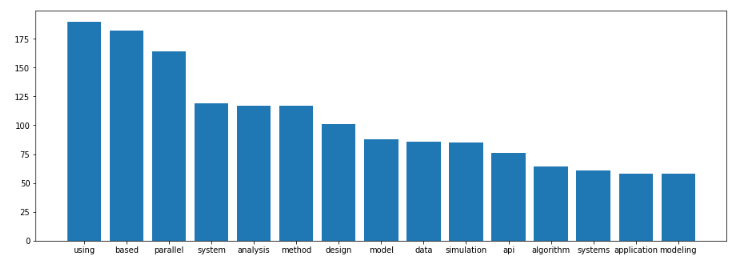
\includegraphics[width=0.5\textwidth]{images/CapturaTL.png}
  \hspace{3cm}
  \begin{center}
  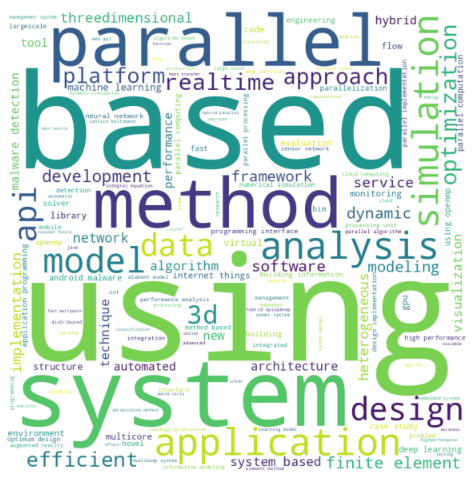
\includegraphics[ height=5cm, width=5cm]{images/CapturaTL2.png}
  \end{center}


\subsection{Analisis de Keyword}

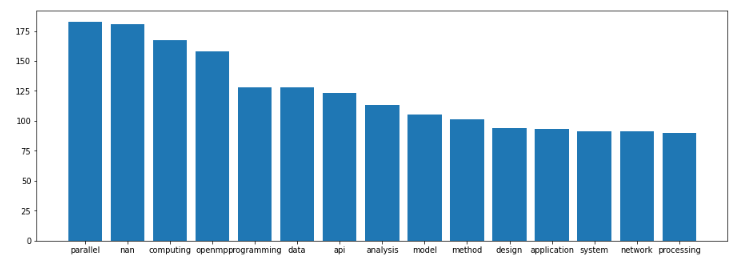
\includegraphics[width=0.5\textwidth]{images/CapturaKW.png}
  \hspace{3cm}
  \begin{center}
  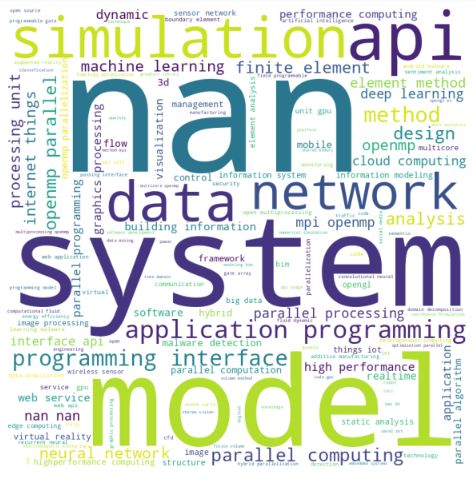
\includegraphics[ height=5cm, width=5cm]{images/CapturaKW2.png}
  \end{center}

\subsection{Analisis de Abstract}

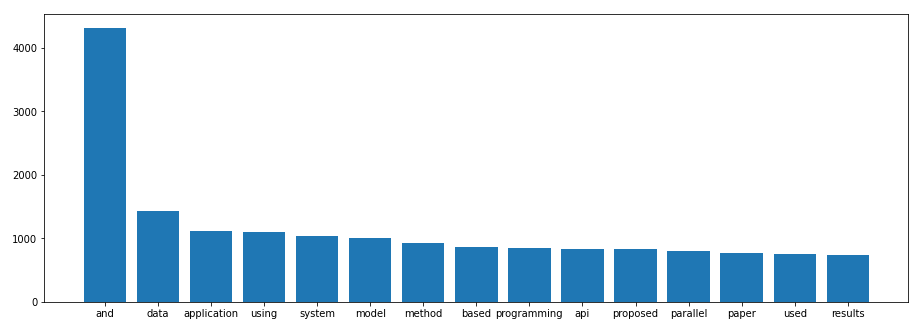
\includegraphics[width=0.5\textwidth]{images/graficakw.png}
  \hspace{3cm}
  \begin{center}
  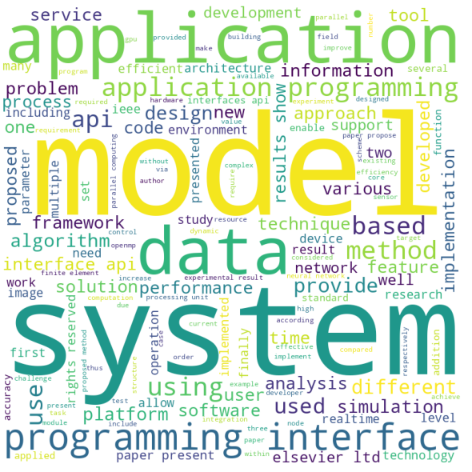
\includegraphics[ height=5cm, width=5cm]{images/grafica2.png}
  \end{center}


\subsection{Ranking de plabras clave para la construction del nuevo filtro}

Las palabras usadaas fueron using, system y data


\subsection{Query Resultante}

TITLE-ABS-KEY ( api  AND  using  AND  system  AND  data )  AND  PUBYEAR  >  2010  AND  PUBYEAR  <  2024  AND  ( LIMIT-TO ( SUBJAREA ,  "ENGI" ) )  AND  ( LIMIT-TO ( DOCTYPE ,  "ar" ) )  AND  ( LIMIT-TO ( LANGUAGE ,  "English" ) )  AND  ( LIMIT-TO ( EXACTKEYWORD ,  "Application Programming Interfaces (API)" ) )  AND  (  LIMIT-TO ( OA ,  "publisherfullgold" ) )  AND  ( EXCLUDE ( SUBJAREA ,  "PHYS" ) ) .

% Conclusiones
\section{Conclusiones}

Las API se han convertido en una herramienta fundamental para el desarrollo de software en la actualidad, permitiendo una mayor eficiencia y rapidez en la creación de aplicaciones y sistemas complejos.

La literatura revisada destaca la importancia de la implementación adecuada de las API, así como su integración con otros sistemas y plataformas.

La seguridad y la privacidad son temas críticos en el uso de las API, y se necesitan medidas específicas para garantizar la protección de datos y la prevención de vulnerabilidades.

Por último, el análisis bibliográfico tiene una gran importancia para obtener los temas y palabras más relevantes referentes al tema que se esté buscando. De igual manera, se obtiene una ayuda visual, la cual son las gráficas, obteniendo con mayor facilidad la información.


\vspace{12pt}
\end{document}
